\documentclass{scrartcl}
\usepackage[utf8]{inputenc}
\usepackage{graphicx}
\usepackage{adjustbox}
\usepackage{amsmath}
\usepackage{float}
\usepackage{siunitx}
\sisetup{
  per-mode=symbol,
  separate-uncertainty
}
\usepackage{hyperref}
\hypersetup{
    colorlinks=true,
    linkcolor=blue,
    filecolor=magenta,      
    urlcolor=cyan,    
    }
\usepackage{authblk}

\usepackage{minted}

\title{CGL-sheet08}

\author[1]{Robin Kühnberger}
\author[2]{Felix Naraschewski}

\affil[1]{University Stuttgart}
\affil[2]{University Stuttgart}

\date{\today}

\begin{document}
\maketitle
\tableofcontents

\section{Numpy-arrays}

\inputminted[breaklines]{python3}{numpy-arrays.py}


\section{Plotten einer gedämpften harmonischen Schwingung mit matplotlib und argparse}

\subsection{Teil 1: Implementierung und Darstellung}

\inputminted[breaklines]{python3}{damped_oscillation.py}

\begin{figure}[H]
  \centering
  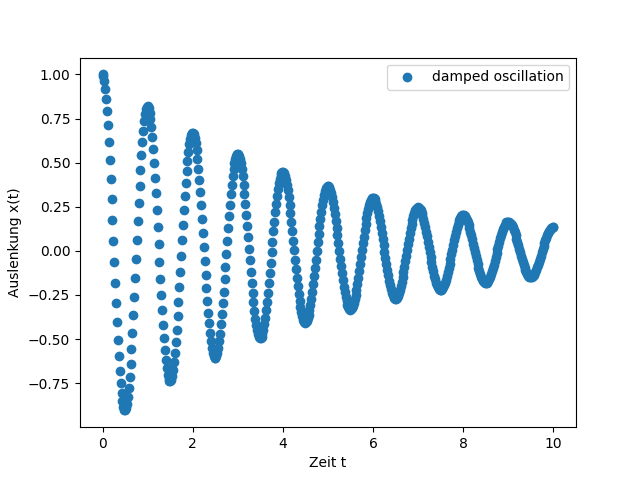
\includegraphics[width=1\textwidth]{damped_oscillation.png}
  \caption{Scatter Plot}
  \label{img:01}
\end{figure}

\subsection{Teil 2: Erweiterung mit argparse (Kommandozeilen-Argumente)}

\inputminted[breaklines]{python3}{damped_oscillator_argparse.py}

\begin{figure}[H]
  \centering
  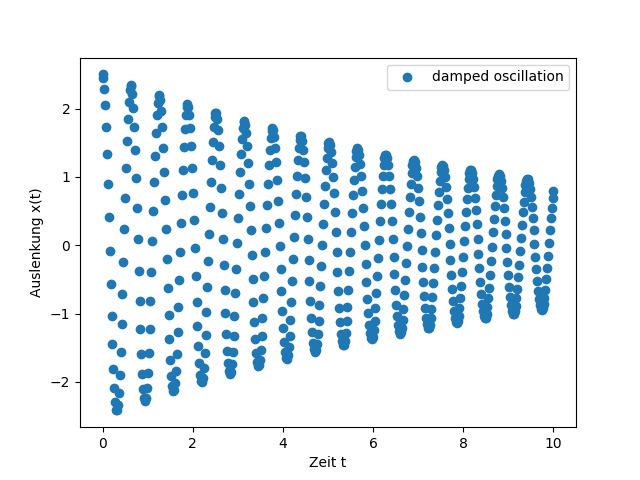
\includegraphics[width=1\textwidth]{damped_oscillator_argparse.png}
  \caption{Colorbar Plot}
  \label{img:02}
\end{figure}

\section{Array-Slicing}

\inputminted[breaklines]{python3}{array-slicing.py}

\begin{figure}[H]
  \centering
  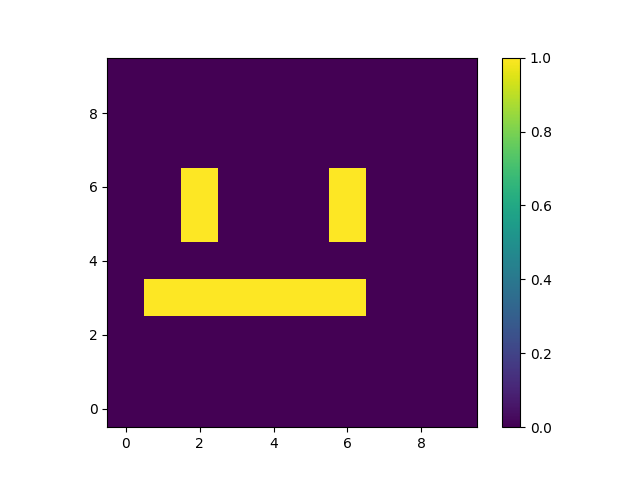
\includegraphics[width=1\textwidth]{array-slicing.png}
  \caption{Colorbar Plot}
  \label{img:03}
\end{figure}

\begin{figure}[H]
  \centering
  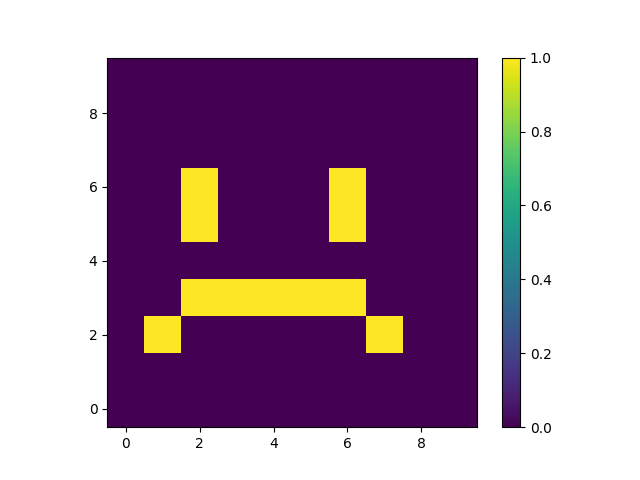
\includegraphics[width=1\textwidth]{array-slicing-sad.png}
  \caption{Colorbar Plot}
  \label{img:04}
\end{figure}


%\section*{Quellen}
%\bibliographystyle{plain}
%\bibliography{bibliography}

\listoffigures
%\listoftables

\end{document}